% Options for packages loaded elsewhere
\PassOptionsToPackage{unicode}{hyperref}
\PassOptionsToPackage{hyphens}{url}
%
\documentclass[
]{book}
\usepackage{amsmath,amssymb}
\usepackage{iftex}
\ifPDFTeX
  \usepackage[T1]{fontenc}
  \usepackage[utf8]{inputenc}
  \usepackage{textcomp} % provide euro and other symbols
\else % if luatex or xetex
  \usepackage{unicode-math} % this also loads fontspec
  \defaultfontfeatures{Scale=MatchLowercase}
  \defaultfontfeatures[\rmfamily]{Ligatures=TeX,Scale=1}
\fi
\usepackage{lmodern}
\ifPDFTeX\else
  % xetex/luatex font selection
\fi
% Use upquote if available, for straight quotes in verbatim environments
\IfFileExists{upquote.sty}{\usepackage{upquote}}{}
\IfFileExists{microtype.sty}{% use microtype if available
  \usepackage[]{microtype}
  \UseMicrotypeSet[protrusion]{basicmath} % disable protrusion for tt fonts
}{}
\makeatletter
\@ifundefined{KOMAClassName}{% if non-KOMA class
  \IfFileExists{parskip.sty}{%
    \usepackage{parskip}
  }{% else
    \setlength{\parindent}{0pt}
    \setlength{\parskip}{6pt plus 2pt minus 1pt}}
}{% if KOMA class
  \KOMAoptions{parskip=half}}
\makeatother
\usepackage{xcolor}
\usepackage{color}
\usepackage{fancyvrb}
\newcommand{\VerbBar}{|}
\newcommand{\VERB}{\Verb[commandchars=\\\{\}]}
\DefineVerbatimEnvironment{Highlighting}{Verbatim}{commandchars=\\\{\}}
% Add ',fontsize=\small' for more characters per line
\usepackage{framed}
\definecolor{shadecolor}{RGB}{248,248,248}
\newenvironment{Shaded}{\begin{snugshade}}{\end{snugshade}}
\newcommand{\AlertTok}[1]{\textcolor[rgb]{0.94,0.16,0.16}{#1}}
\newcommand{\AnnotationTok}[1]{\textcolor[rgb]{0.56,0.35,0.01}{\textbf{\textit{#1}}}}
\newcommand{\AttributeTok}[1]{\textcolor[rgb]{0.13,0.29,0.53}{#1}}
\newcommand{\BaseNTok}[1]{\textcolor[rgb]{0.00,0.00,0.81}{#1}}
\newcommand{\BuiltInTok}[1]{#1}
\newcommand{\CharTok}[1]{\textcolor[rgb]{0.31,0.60,0.02}{#1}}
\newcommand{\CommentTok}[1]{\textcolor[rgb]{0.56,0.35,0.01}{\textit{#1}}}
\newcommand{\CommentVarTok}[1]{\textcolor[rgb]{0.56,0.35,0.01}{\textbf{\textit{#1}}}}
\newcommand{\ConstantTok}[1]{\textcolor[rgb]{0.56,0.35,0.01}{#1}}
\newcommand{\ControlFlowTok}[1]{\textcolor[rgb]{0.13,0.29,0.53}{\textbf{#1}}}
\newcommand{\DataTypeTok}[1]{\textcolor[rgb]{0.13,0.29,0.53}{#1}}
\newcommand{\DecValTok}[1]{\textcolor[rgb]{0.00,0.00,0.81}{#1}}
\newcommand{\DocumentationTok}[1]{\textcolor[rgb]{0.56,0.35,0.01}{\textbf{\textit{#1}}}}
\newcommand{\ErrorTok}[1]{\textcolor[rgb]{0.64,0.00,0.00}{\textbf{#1}}}
\newcommand{\ExtensionTok}[1]{#1}
\newcommand{\FloatTok}[1]{\textcolor[rgb]{0.00,0.00,0.81}{#1}}
\newcommand{\FunctionTok}[1]{\textcolor[rgb]{0.13,0.29,0.53}{\textbf{#1}}}
\newcommand{\ImportTok}[1]{#1}
\newcommand{\InformationTok}[1]{\textcolor[rgb]{0.56,0.35,0.01}{\textbf{\textit{#1}}}}
\newcommand{\KeywordTok}[1]{\textcolor[rgb]{0.13,0.29,0.53}{\textbf{#1}}}
\newcommand{\NormalTok}[1]{#1}
\newcommand{\OperatorTok}[1]{\textcolor[rgb]{0.81,0.36,0.00}{\textbf{#1}}}
\newcommand{\OtherTok}[1]{\textcolor[rgb]{0.56,0.35,0.01}{#1}}
\newcommand{\PreprocessorTok}[1]{\textcolor[rgb]{0.56,0.35,0.01}{\textit{#1}}}
\newcommand{\RegionMarkerTok}[1]{#1}
\newcommand{\SpecialCharTok}[1]{\textcolor[rgb]{0.81,0.36,0.00}{\textbf{#1}}}
\newcommand{\SpecialStringTok}[1]{\textcolor[rgb]{0.31,0.60,0.02}{#1}}
\newcommand{\StringTok}[1]{\textcolor[rgb]{0.31,0.60,0.02}{#1}}
\newcommand{\VariableTok}[1]{\textcolor[rgb]{0.00,0.00,0.00}{#1}}
\newcommand{\VerbatimStringTok}[1]{\textcolor[rgb]{0.31,0.60,0.02}{#1}}
\newcommand{\WarningTok}[1]{\textcolor[rgb]{0.56,0.35,0.01}{\textbf{\textit{#1}}}}
\usepackage{longtable,booktabs,array}
\usepackage{calc} % for calculating minipage widths
% Correct order of tables after \paragraph or \subparagraph
\usepackage{etoolbox}
\makeatletter
\patchcmd\longtable{\par}{\if@noskipsec\mbox{}\fi\par}{}{}
\makeatother
% Allow footnotes in longtable head/foot
\IfFileExists{footnotehyper.sty}{\usepackage{footnotehyper}}{\usepackage{footnote}}
\makesavenoteenv{longtable}
\usepackage{graphicx}
\makeatletter
\def\maxwidth{\ifdim\Gin@nat@width>\linewidth\linewidth\else\Gin@nat@width\fi}
\def\maxheight{\ifdim\Gin@nat@height>\textheight\textheight\else\Gin@nat@height\fi}
\makeatother
% Scale images if necessary, so that they will not overflow the page
% margins by default, and it is still possible to overwrite the defaults
% using explicit options in \includegraphics[width, height, ...]{}
\setkeys{Gin}{width=\maxwidth,height=\maxheight,keepaspectratio}
% Set default figure placement to htbp
\makeatletter
\def\fps@figure{htbp}
\makeatother
\setlength{\emergencystretch}{3em} % prevent overfull lines
\providecommand{\tightlist}{%
  \setlength{\itemsep}{0pt}\setlength{\parskip}{0pt}}
\setcounter{secnumdepth}{5}
\usepackage{booktabs}
\usepackage[scale = 0.9]{geometry}
\ifLuaTeX
  \usepackage{selnolig}  % disable illegal ligatures
\fi
\usepackage[]{natbib}
\bibliographystyle{plainnat}
\IfFileExists{bookmark.sty}{\usepackage{bookmark}}{\usepackage{hyperref}}
\IfFileExists{xurl.sty}{\usepackage{xurl}}{} % add URL line breaks if available
\urlstyle{same}
\hypersetup{
  pdftitle={Financial Econometrics - Tutorials},
  pdfauthor={Alessandro Ciancetta},
  hidelinks,
  pdfcreator={LaTeX via pandoc}}

\title{Financial Econometrics - Tutorials}
\author{Alessandro Ciancetta}
\date{Last update: January 19, 2024}

\begin{document}
\maketitle

{
\setcounter{tocdepth}{1}
\tableofcontents
}
\hypertarget{about}{%
\chapter*{About}\label{about}}
\addcontentsline{toc}{chapter}{About}

TA materials for the Financial Econometrics course held by Prof.~Christian Brownlees at the Barcelona School of Economics.

\begin{center}\includegraphics[width=1\linewidth]{pic_finmetrics} \end{center}

\hypertarget{session01}{%
\chapter{Introduction to time series}\label{session01}}

\hypertarget{stochastic-processes-and-dependence}{%
\section{Stochastic processes and dependence}\label{stochastic-processes-and-dependence}}

Stochastic processes are a tool for modeling dependence in consecutive random variables \(\{\dots, Y_{-2}, Y_{-1}, Y_{0}, Y_{1}, Y_{2} \dots\}\). However, in practice, when we observe an empirical time series we are considering \emph{one, truncated} realization of the stochastic process, \(\{y_1, y_2, \dots, y_T\}\). As it is easy to imagine, this can cause some issues in studying the properties of an empirical time series. First, because we can only study the \emph{finite} dimensional distribution of the process. Second, because our task is to learn something about the process by knowing only one realization of it.

To overcome this limitations we need assumptions. In particular, two common assumptions in time series analysis are, loosely speaking:

\begin{itemize}
\item
  stationarity: the observed values in the sequence come from the same distribution, so that it is possible to learn from the past observations and to generalize the results to the entire, infinite stochastic process
\item
  ergodicity: values observed far away in time can be considered as independent, and hence if we have enough observations the empirical time series is representative of the entire distribution of the stochastic process
\end{itemize}

Under these (or similar) assumptions, we can use the observations from a single empirical time series to learn the parameters of our models.

\hypertarget{stationarity}{%
\subsection*{Stationarity}\label{stationarity}}
\addcontentsline{toc}{subsection}{Stationarity}

Consider the example in the plot below. If we had only observations laying between two changepoints we would not be able to retrieve the dynamics of the underlying process. For instance, if we observed a series ending before the first changepoint, we would have no information about the future realizations of the process. Indeed, future observations would come from different distributions that we could not learn from available information.

\begin{Shaded}
\begin{Highlighting}[]
\DocumentationTok{\#\# Example 1: non{-}stationary process}
\CommentTok{\# simulation}
\NormalTok{t\_max }\OtherTok{\textless{}{-}} \DecValTok{500}
\NormalTok{y }\OtherTok{\textless{}{-}} \FunctionTok{rep}\NormalTok{(}\ConstantTok{NA}\NormalTok{, t\_max)}
\ControlFlowTok{for}\NormalTok{ (t }\ControlFlowTok{in} \DecValTok{1}\SpecialCharTok{:}\NormalTok{t\_max) \{}
  \ControlFlowTok{if}\NormalTok{ (t}\SpecialCharTok{\textless{}=}\DecValTok{100}\NormalTok{) \{}
\NormalTok{    y[t] }\OtherTok{\textless{}{-}} \FunctionTok{rnorm}\NormalTok{(}\DecValTok{1}\NormalTok{, }\AttributeTok{mean =} \DecValTok{0}\NormalTok{, }\AttributeTok{sd =} \FloatTok{0.1}\NormalTok{)}
\NormalTok{  \}}
  \ControlFlowTok{if}\NormalTok{ (t}\SpecialCharTok{\textgreater{}}\DecValTok{100} \SpecialCharTok{\&}\NormalTok{ t}\SpecialCharTok{\textless{}=}\DecValTok{250}\NormalTok{) \{}
\NormalTok{    y[t] }\OtherTok{\textless{}{-}} \FunctionTok{rnorm}\NormalTok{(}\DecValTok{1}\NormalTok{, }\AttributeTok{mean =} \FloatTok{0.5}\NormalTok{, }\AttributeTok{sd =} \FloatTok{0.1}\NormalTok{)}
\NormalTok{  \}}
  \ControlFlowTok{if}\NormalTok{ (t}\SpecialCharTok{\textgreater{}}\DecValTok{250} \SpecialCharTok{\&}\NormalTok{ t}\SpecialCharTok{\textless{}=}\DecValTok{400}\NormalTok{) \{}
\NormalTok{    y[t] }\OtherTok{\textless{}{-}} \FunctionTok{rnorm}\NormalTok{(}\DecValTok{1}\NormalTok{, }\AttributeTok{mean =} \DecValTok{0}\NormalTok{, }\AttributeTok{sd =} \FloatTok{0.2}\NormalTok{)}
\NormalTok{  \}}
  \ControlFlowTok{if}\NormalTok{ (t}\SpecialCharTok{\textgreater{}}\DecValTok{400} \SpecialCharTok{\&}\NormalTok{ t}\SpecialCharTok{\textless{}=}\NormalTok{t\_max) \{}
\NormalTok{    y[t] }\OtherTok{\textless{}{-}} \FloatTok{0.01}\SpecialCharTok{*}\NormalTok{(t}\DecValTok{{-}400}\NormalTok{) }\SpecialCharTok{+} \FunctionTok{rnorm}\NormalTok{(}\DecValTok{1}\NormalTok{, }\AttributeTok{mean =} \SpecialCharTok{{-}}\FloatTok{0.2}\NormalTok{, }\AttributeTok{sd =} \FloatTok{0.02}\NormalTok{)}
\NormalTok{  \}}
\NormalTok{\}}
\CommentTok{\# plot}
\FunctionTok{plot.ts}\NormalTok{(y, }\AttributeTok{main =} \StringTok{"Non{-}stationary process"}\NormalTok{, }\AttributeTok{xaxt =} \StringTok{"n"}\NormalTok{)}
\FunctionTok{abline}\NormalTok{(}\AttributeTok{v =} \FunctionTok{c}\NormalTok{(}\DecValTok{100}\NormalTok{, }\DecValTok{250}\NormalTok{, }\DecValTok{400}\NormalTok{), }\AttributeTok{lty =} \DecValTok{2}\NormalTok{)}
\FunctionTok{axis}\NormalTok{(}\DecValTok{1}\NormalTok{, }\AttributeTok{at=}\FunctionTok{c}\NormalTok{(}\DecValTok{100}\NormalTok{, }\DecValTok{250}\NormalTok{, }\DecValTok{400}\NormalTok{),}
     \AttributeTok{labels =} \FunctionTok{c}\NormalTok{(}\StringTok{"Changepoint 1"}\NormalTok{, }\StringTok{"Changepoint 2"}\NormalTok{, }\StringTok{"Changepoint 3"}\NormalTok{))}
\end{Highlighting}
\end{Shaded}

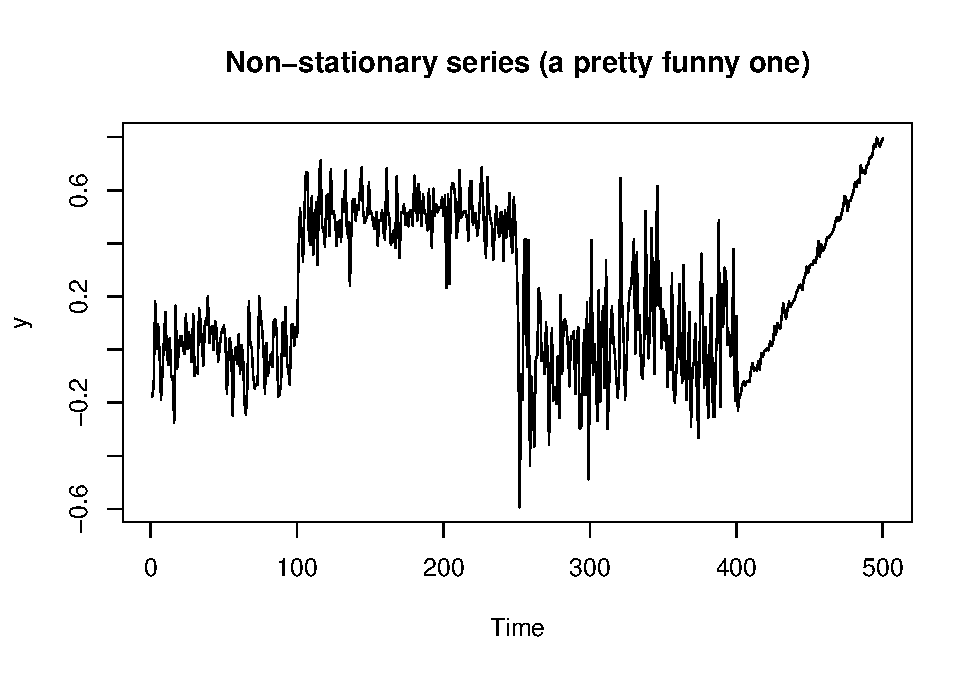
\includegraphics{_main_files/figure-latex/unnamed-chunk-3-1.pdf}

\hypertarget{ergodicity}{%
\subsection*{Ergodicity}\label{ergodicity}}
\addcontentsline{toc}{subsection}{Ergodicity}

Let \(\{z_t\}_{t = 1}^{T} \stackrel{iid}{\sim} \mathcal{N}(0, 1)\). Consider the two following data-generating processes:

\[
\begin{aligned}
y_t &= U_0 + 0.25z_t, \quad \text{with  } U_0 \sim \mathcal{N}(0, 100) \\[1ex]
x_t &= z_t + z_{t-1}
\end{aligned}
\]

We have:

\[
\begin{aligned}
\mathbb{E}[y_t] &= \mathbb{E}[x_t] = 0 \\[1em]
\text{cov}(y_t, y_{t-k}) &= 
\begin{cases}
100+0.25^2 & k = 0 \\
100 & k \neq 0
\end{cases} \\[1ex]
\text{cov}(x_t, x_{t-k}) &= 
\begin{cases}
2 & k = 0 \\
1 & k = 1 \\
0 & k \geq 2
\end{cases}
\end{aligned}
\]

We now simulate the two data generating processes in \texttt{R}. We want to draw many sequences \(\{y_1, \dots, y_T\}^{(s)}, \{x_1, \dots, x_T\}^{(s)}\) for \(s = 1, \dots, S\) simulations to assess whether observing a single time series is enough to estimate the mean of the processes.

\begin{Shaded}
\begin{Highlighting}[]
\DocumentationTok{\#\# Example 2: weak dependence}

\DocumentationTok{\#\# Simulate process y\_t}
\CommentTok{\# initialize TxS matrix to store result }
\CommentTok{\# (each column is a simulated time series \{y\_1, ..., y\_T\}\^{}(s) )}
\NormalTok{nsim }\OtherTok{\textless{}{-}} \DecValTok{3}
\NormalTok{y\_list }\OtherTok{\textless{}{-}} \FunctionTok{matrix}\NormalTok{(}\FunctionTok{rep}\NormalTok{(}\ConstantTok{NA}\NormalTok{, nsim}\SpecialCharTok{*}\NormalTok{t\_max), }\AttributeTok{nrow =}\NormalTok{ t\_max, }\AttributeTok{ncol =}\NormalTok{ nsim)}
\CommentTok{\# simulation}
\ControlFlowTok{for}\NormalTok{ (sim }\ControlFlowTok{in} \DecValTok{1}\SpecialCharTok{:}\NormalTok{nsim) \{}
  \FunctionTok{set.seed}\NormalTok{(sim}\SpecialCharTok{+}\DecValTok{123}\NormalTok{)}
\NormalTok{  U0 }\OtherTok{\textless{}{-}} \FunctionTok{rnorm}\NormalTok{(}\DecValTok{1}\NormalTok{, }\AttributeTok{sd =} \DecValTok{10}\NormalTok{)}
\NormalTok{  z  }\OtherTok{\textless{}{-}} \FunctionTok{rnorm}\NormalTok{(t\_max)}
\NormalTok{  y\_list[,sim] }\OtherTok{\textless{}{-}}\NormalTok{ U0 }\SpecialCharTok{+} \FloatTok{0.25}\SpecialCharTok{*}\NormalTok{z}
\NormalTok{\}}
\end{Highlighting}
\end{Shaded}

As the plot below shows, if we observe a single simulated time series we cannot correctly estimate the mean of the process \(\mathbb{E}[y_t]\) using the sample mean \(\bar{y}_T\). What the sample mean is actually estimating in this case is the \emph{conditional} expctation of \(y_t\) given the specific draw of the random intercept \(U_0\) in simulation \(s\): \(\mathbb{E}\left[y_t | U_0 = U_0^{(s)}\right] = U_0^{(s)}\). Notice that in this case, if we observe a new point for stochastic process \(y_t\) (green points in the plot) we are likely not able to forecast it correctly based on the previous observations of a single time series.

\begin{Shaded}
\begin{Highlighting}[]
\CommentTok{\# plot}
\FunctionTok{plot.ts}\NormalTok{(y\_list[,}\DecValTok{1}\NormalTok{], }\AttributeTok{ylim =} \FunctionTok{c}\NormalTok{(}\SpecialCharTok{{-}}\DecValTok{25}\NormalTok{, }\DecValTok{25}\NormalTok{), }\AttributeTok{main =} \StringTok{"Realizations of non{-}ergodic series"}\NormalTok{, }\AttributeTok{ylab =} \StringTok{"y"}\NormalTok{)}
\FunctionTok{lines}\NormalTok{(y\_list[,}\DecValTok{2}\NormalTok{], }\AttributeTok{col =} \StringTok{"steelblue"}\NormalTok{)}
\FunctionTok{lines}\NormalTok{(y\_list[,}\DecValTok{3}\NormalTok{], }\AttributeTok{col =} \StringTok{"tomato"}\NormalTok{)}
\ControlFlowTok{for}\NormalTok{ (point }\ControlFlowTok{in} \DecValTok{1}\SpecialCharTok{:}\DecValTok{100}\NormalTok{)\{}
  \FunctionTok{points}\NormalTok{(}\AttributeTok{x =} \DecValTok{501}\NormalTok{, }\FunctionTok{rnorm}\NormalTok{(}\DecValTok{1}\NormalTok{, }\DecValTok{0}\NormalTok{, }\DecValTok{10}\NormalTok{)}\SpecialCharTok{+}\FunctionTok{rnorm}\NormalTok{(}\DecValTok{1}\NormalTok{, }\DecValTok{0}\NormalTok{, }\DecValTok{1}\NormalTok{), }\AttributeTok{col =} \StringTok{"darkgreen"}\NormalTok{, }\AttributeTok{pch =} \DecValTok{4}\NormalTok{)}
\NormalTok{\}}
\FunctionTok{abline}\NormalTok{(}\AttributeTok{h =} \DecValTok{0}\NormalTok{, }\AttributeTok{col =} \StringTok{"black"}\NormalTok{, }\AttributeTok{lwd =} \DecValTok{2}\NormalTok{, }\AttributeTok{lty =} \DecValTok{2}\NormalTok{)}
\end{Highlighting}
\end{Shaded}

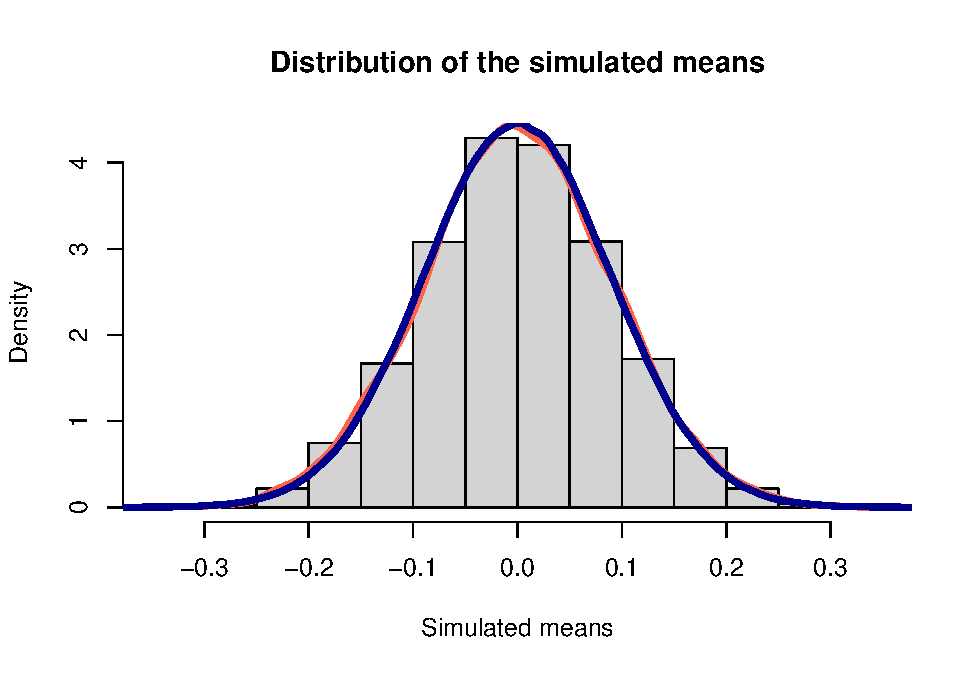
\includegraphics{_main_files/figure-latex/unnamed-chunk-5-1.pdf}

We now turn to process \(x_t\).

\begin{Shaded}
\begin{Highlighting}[]
\DocumentationTok{\#\# Simulate process x\_t}
\CommentTok{\# initialize object to store result}
\NormalTok{nsim }\OtherTok{\textless{}{-}} \DecValTok{10000}
\NormalTok{x\_list }\OtherTok{\textless{}{-}} \FunctionTok{matrix}\NormalTok{(}\FunctionTok{rep}\NormalTok{(}\ConstantTok{NA}\NormalTok{, nsim}\SpecialCharTok{*}\NormalTok{t\_max), }\AttributeTok{nrow =}\NormalTok{ t\_max, }\AttributeTok{ncol =}\NormalTok{ nsim)}
\CommentTok{\# simulation}
\ControlFlowTok{for}\NormalTok{ (sim }\ControlFlowTok{in} \DecValTok{1}\SpecialCharTok{:}\NormalTok{nsim) \{}
  \FunctionTok{set.seed}\NormalTok{(sim}\SpecialCharTok{+}\DecValTok{123}\NormalTok{)}
\NormalTok{  z  }\OtherTok{\textless{}{-}} \FunctionTok{rnorm}\NormalTok{(t\_max}\SpecialCharTok{+}\DecValTok{1}\NormalTok{)}
\NormalTok{  x\_list[,sim] }\OtherTok{\textless{}{-}}\NormalTok{ z[}\DecValTok{2}\SpecialCharTok{:}\NormalTok{(t\_max}\SpecialCharTok{+}\DecValTok{1}\NormalTok{)] }\SpecialCharTok{+}\NormalTok{ z[}\DecValTok{1}\SpecialCharTok{:}\NormalTok{t\_max]}
\NormalTok{\}}
\end{Highlighting}
\end{Shaded}

All the simulated time series have mean zero in this case. As a consequence, we can use the sample mean \(\bar{x}_T\) obtained from a single time series to estimate the (unconditional) mean of the process \(\mathbb{E}[x_t]\).

\begin{Shaded}
\begin{Highlighting}[]
\CommentTok{\# plot}
\FunctionTok{plot.ts}\NormalTok{(x\_list[,}\DecValTok{1}\NormalTok{], }\AttributeTok{ylim =} \FunctionTok{c}\NormalTok{(}\FunctionTok{min}\NormalTok{(x\_list), }\FunctionTok{max}\NormalTok{(x\_list)), }
        \AttributeTok{main =} \StringTok{"Realizations of ergodic series"}\NormalTok{, }\AttributeTok{ylab =} \StringTok{"x"}\NormalTok{)}
\FunctionTok{lines}\NormalTok{(x\_list[,}\DecValTok{2}\NormalTok{], }\AttributeTok{col =} \StringTok{"steelblue"}\NormalTok{)}
\FunctionTok{lines}\NormalTok{(x\_list[,}\DecValTok{3}\NormalTok{], }\AttributeTok{col =} \StringTok{"tomato"}\NormalTok{)}
\FunctionTok{abline}\NormalTok{(}\AttributeTok{h =} \DecValTok{0}\NormalTok{, }\AttributeTok{col =} \StringTok{"black"}\NormalTok{, }\AttributeTok{lwd =} \DecValTok{2}\NormalTok{, }\AttributeTok{lty =} \DecValTok{2}\NormalTok{)}
\end{Highlighting}
\end{Shaded}

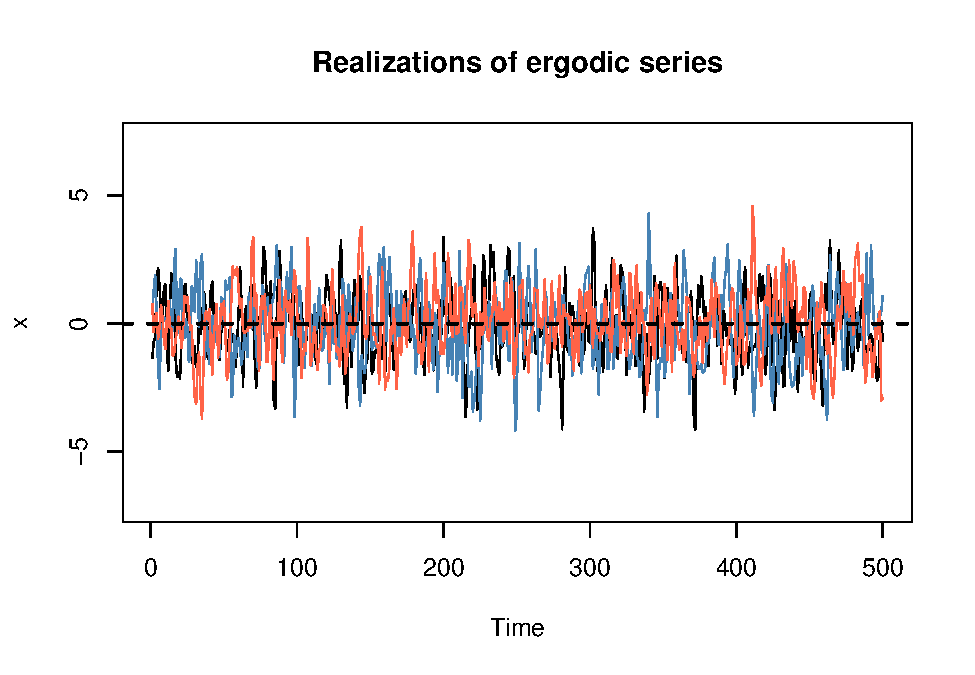
\includegraphics{_main_files/figure-latex/unnamed-chunk-7-1.pdf}

\hypertarget{asymptotic-results}{%
\section{Asymptotic results}\label{asymptotic-results}}

The problem with the series \(\{y_t\}\) in the previous example is that the autocovariance function does not decay as the lag order increases. Loosely speaking, the series gets stuck in the trajectory given by the initial draw of \(U_0\) and does not revert to the true mean of the stochastic process. The main consequence is that we cannot learn the mean of the process by taking the average of the observations in a single realized time series.

It is true in general that some conditions on the rate of decay of the autocovariance are required to recover the mean of the process. For example, the Law of Large Numbers (LLN) guarantees that the sample mean converges in probability to the true mean under the assumption that the autocovariances are absolutely summable:

\[
\sum_{k=0}^\infty |\gamma_k| < \infty
\]

Notice that in the case of \(\{y_t\}\) above instead \(\sum_{k=0}^\infty |\gamma_k| = \infty\). On the contrary, \(\{x_t\}\) satisfies both the conditions of the LLN and of the Central Limit Theorem (CLT). The condition for the latter is that \(\{\phi_k\}_{k=0}^\infty\) is absolutely summable in \(x_t = \mu_x + \sum_{k=0}^\infty\phi_k z_{t-k} = z_t + z_{t-1}\), which is trivially verified. Therefore, since \(\mu_x = 0\),

\[
\sqrt{T} \ \bar{x}_T  \ \xrightarrow{d} \ \mathcal{N}(0, \sigma^2_{LR}),
\]

with \(\sigma^2_{LR} = \sum_{k=-\infty}^\infty \gamma_k = \text{Var}(x_t) + 2\sum_{k=1}^\infty \gamma_k\).

\begin{Shaded}
\begin{Highlighting}[]
\DocumentationTok{\#\# Example 3: central limit theorem}
\NormalTok{x\_empirical }\OtherTok{\textless{}{-}}\NormalTok{ x\_list[,}\DecValTok{9}\NormalTok{]}
\NormalTok{x\_means }\OtherTok{\textless{}{-}} \FunctionTok{colMeans}\NormalTok{(x\_list)}
\NormalTok{x\_theory\_variance }\OtherTok{\textless{}{-}} \DecValTok{4}  \CommentTok{\# long run variance}
\NormalTok{x\_empir\_variance }\OtherTok{\textless{}{-}} \FunctionTok{var}\NormalTok{(x\_empirical) }\SpecialCharTok{+} \DecValTok{2}\SpecialCharTok{*}\NormalTok{(}\FunctionTok{cov}\NormalTok{(x\_empirical[}\DecValTok{1}\SpecialCharTok{:}\NormalTok{(t\_max}\DecValTok{{-}1}\NormalTok{)], x\_empirical[}\DecValTok{2}\SpecialCharTok{:}\NormalTok{t\_max]))}

\FunctionTok{rbind}\NormalTok{(}\AttributeTok{empirical\_variance =}\NormalTok{ x\_empir\_variance,}
      \AttributeTok{simulated\_variance =} \FunctionTok{var}\NormalTok{(x\_means}\SpecialCharTok{*}\FunctionTok{sqrt}\NormalTok{(t\_max)),}
      \AttributeTok{theoretical\_variance =}\NormalTok{ x\_theory\_variance)}
\end{Highlighting}
\end{Shaded}

\begin{verbatim}
##                          [,1]
## empirical_variance   4.174614
## simulated_variance   4.050667
## theoretical_variance 4.000000
\end{verbatim}

\begin{Shaded}
\begin{Highlighting}[]
\DocumentationTok{\#\# Plot empirical distribution VS. theoretical distribution}
\FunctionTok{hist}\NormalTok{(x\_means}\SpecialCharTok{*}\FunctionTok{sqrt}\NormalTok{(t\_max), }\AttributeTok{breaks =} \DecValTok{20}\NormalTok{, }\AttributeTok{freq =} \ConstantTok{FALSE}\NormalTok{, }
     \AttributeTok{main =} \StringTok{"Distribution of the simulated means"}\NormalTok{, }
     \AttributeTok{xlab =} \FunctionTok{expression}\NormalTok{(Simulated }\SpecialCharTok{\textasciitilde{}}\NormalTok{ means }\SpecialCharTok{\textasciitilde{}}\NormalTok{ rescaled }\SpecialCharTok{\textasciitilde{}}\NormalTok{ by }\SpecialCharTok{\textasciitilde{}} \FunctionTok{sqrt}\NormalTok{(T)))}
\FunctionTok{lines}\NormalTok{(}\FunctionTok{density}\NormalTok{(x\_means}\SpecialCharTok{*}\FunctionTok{sqrt}\NormalTok{(t\_max)), }\AttributeTok{lwd =} \DecValTok{4}\NormalTok{, }\AttributeTok{col =} \StringTok{"tomato"}\NormalTok{)}
\FunctionTok{lines}\NormalTok{(}\FunctionTok{density}\NormalTok{(}\FunctionTok{rnorm}\NormalTok{(}\FloatTok{1e6}\NormalTok{, }\AttributeTok{mean =} \DecValTok{0}\NormalTok{, }\AttributeTok{sd =} \FunctionTok{sqrt}\NormalTok{(x\_theory\_variance))), }\AttributeTok{lwd =} \DecValTok{4}\NormalTok{, }\AttributeTok{col =} \StringTok{"darkblue"}\NormalTok{)}
\end{Highlighting}
\end{Shaded}

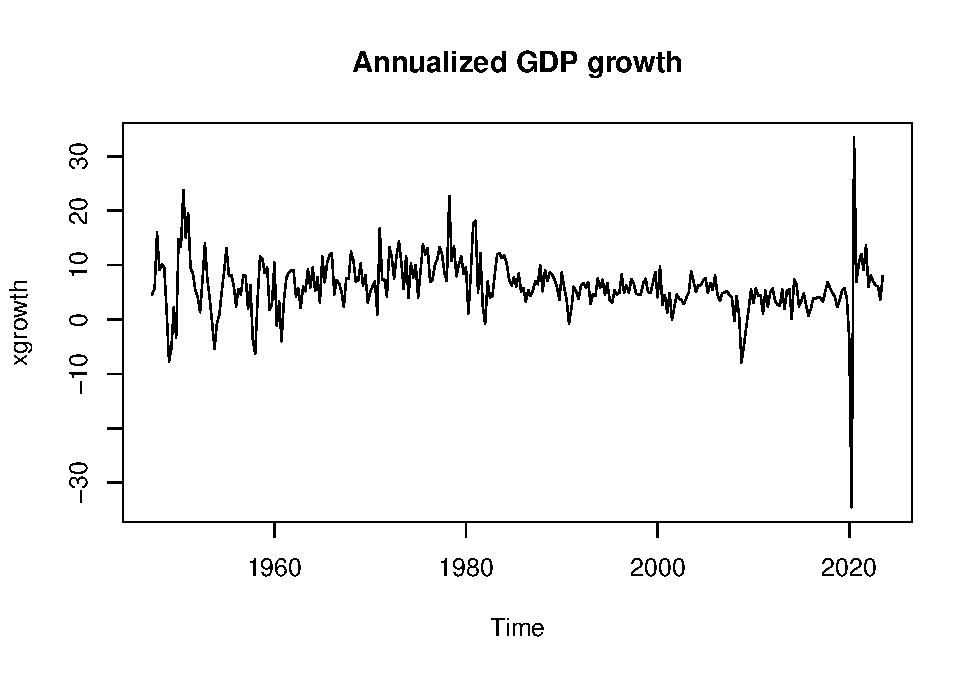
\includegraphics{_main_files/figure-latex/unnamed-chunk-9-1.pdf}

\hypertarget{empirical-moments-and-summary-statistics}{%
\section{Empirical moments and summary statistics}\label{empirical-moments-and-summary-statistics}}

For this example we use the \href{https://fred.stlouisfed.org/series/GDP}{U.S. GDP data}.

\begin{Shaded}
\begin{Highlighting}[]
\NormalTok{x }\OtherTok{\textless{}{-}} \FunctionTok{read.csv}\NormalTok{(}\StringTok{"../data/us{-}gdp.csv"}\NormalTok{)[,}\DecValTok{2}\NormalTok{]}
\NormalTok{x }\OtherTok{\textless{}{-}} \FunctionTok{ts}\NormalTok{(x, }\AttributeTok{start =} \FunctionTok{c}\NormalTok{(}\DecValTok{1947}\NormalTok{, }\DecValTok{1}\NormalTok{), }\AttributeTok{frequency =} \DecValTok{4}\NormalTok{)}
\NormalTok{t\_max }\OtherTok{\textless{}{-}} \FunctionTok{length}\NormalTok{(x)}
\FunctionTok{plot.ts}\NormalTok{(x, }\AttributeTok{main =} \StringTok{"U.S. GDP"}\NormalTok{, }\AttributeTok{ylab =} \StringTok{"Billions of dollars"}\NormalTok{)}
\end{Highlighting}
\end{Shaded}

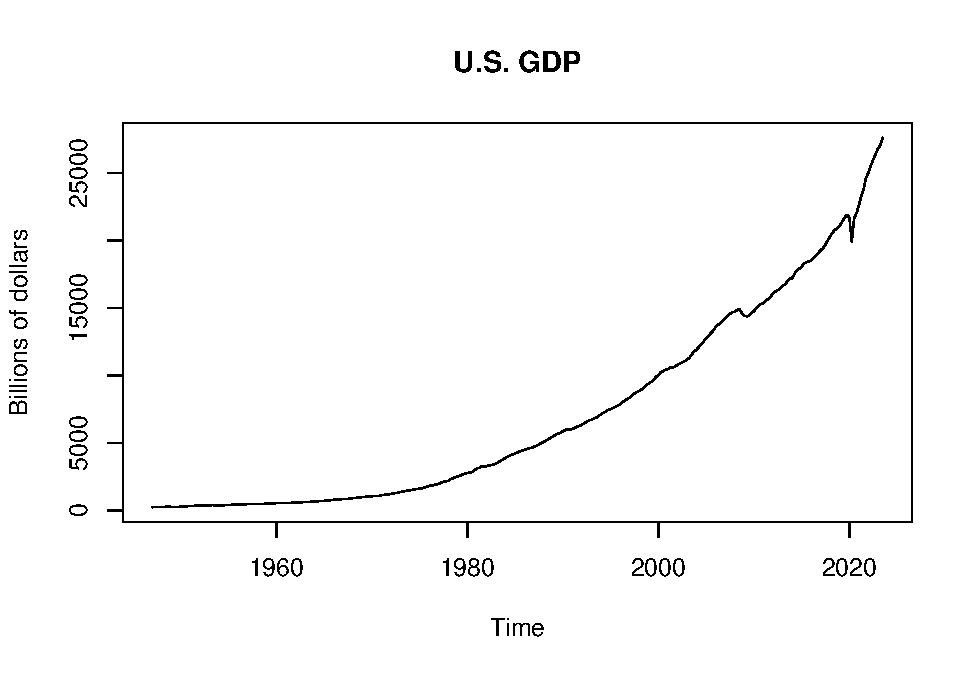
\includegraphics{_main_files/figure-latex/unnamed-chunk-10-1.pdf}

Consider the annualized quarterly growth rates:

\begin{Shaded}
\begin{Highlighting}[]
\CommentTok{\# xgrowth \textless{}{-} ( (x[2:t\_max]/x[1:(t\_max{-}1)])\^{}4 {-} 1 )*100}
\NormalTok{xgrowth }\OtherTok{\textless{}{-}} \DecValTok{4}\SpecialCharTok{*}\FunctionTok{diff}\NormalTok{(}\FunctionTok{log}\NormalTok{(x))}\SpecialCharTok{*}\DecValTok{100}
\NormalTok{xgrowth }\OtherTok{\textless{}{-}} \FunctionTok{ts}\NormalTok{(xgrowth, }\AttributeTok{start =} \FunctionTok{c}\NormalTok{(}\DecValTok{1947}\NormalTok{, }\DecValTok{2}\NormalTok{), }\AttributeTok{frequency =} \DecValTok{4}\NormalTok{)}
\FunctionTok{plot.ts}\NormalTok{(xgrowth, }\AttributeTok{main =} \StringTok{"Annualized GDP growth"}\NormalTok{)}
\end{Highlighting}
\end{Shaded}

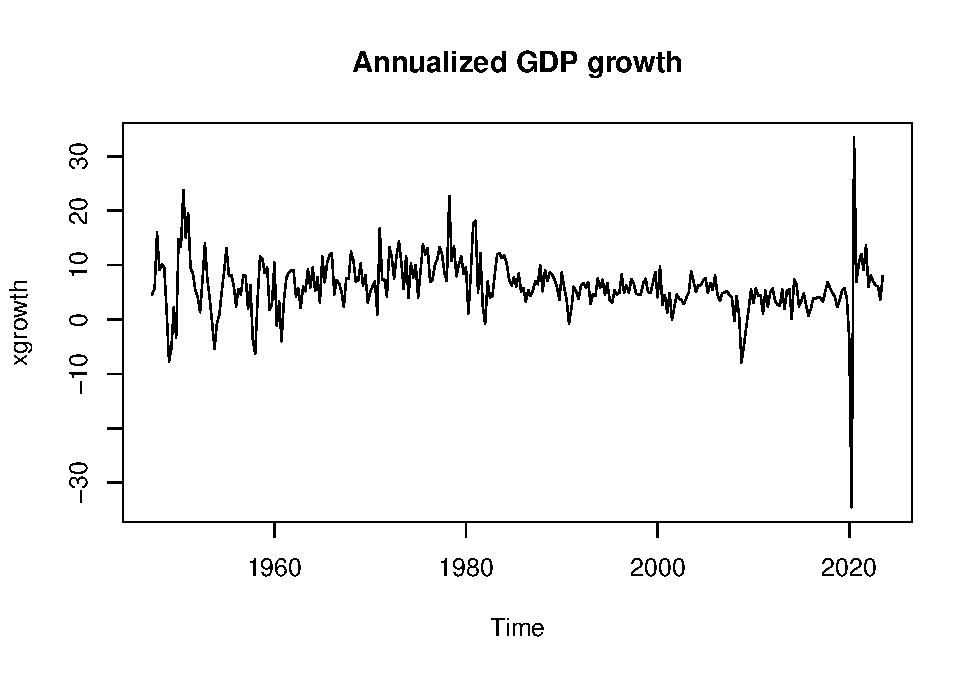
\includegraphics{_main_files/figure-latex/unnamed-chunk-11-1.pdf}

Below we compute some summary statistics for the time series of the U.S. GDP growth rates.

\begin{Shaded}
\begin{Highlighting}[]
\DocumentationTok{\#\# Example 4: empirical moments and summary statistics of the GDP growth}
\FunctionTok{library}\NormalTok{(moments)}
\FunctionTok{rbind}\NormalTok{(}
  \AttributeTok{mean     =} \FunctionTok{mean}\NormalTok{(xgrowth),}
  \AttributeTok{variance =} \FunctionTok{var}\NormalTok{(xgrowth),}
  \AttributeTok{skewness =} \FunctionTok{skewness}\NormalTok{(xgrowth),}
  \AttributeTok{kurtosis =} \FunctionTok{kurtosis}\NormalTok{(xgrowth),}
  \AttributeTok{min      =} \FunctionTok{min}\NormalTok{(xgrowth),}
  \AttributeTok{max      =} \FunctionTok{max}\NormalTok{(xgrowth),}
  \AttributeTok{above\_5  =} \FunctionTok{mean}\NormalTok{(xgrowth }\SpecialCharTok{\textgreater{}} \DecValTok{5}\NormalTok{),}
  \AttributeTok{annualized\_volatility =} \FunctionTok{sqrt}\NormalTok{(}\DecValTok{4}\NormalTok{)}\SpecialCharTok{*}\FunctionTok{sd}\NormalTok{(xgrowth)}
\NormalTok{)}
\end{Highlighting}
\end{Shaded}

\begin{verbatim}
##                              [,1]
## mean                    6.1858847
## variance               26.5117326
## skewness               -0.9793909
## kurtosis               17.9597257
## min                   -34.4929551
## max                    33.4065902
## above_5                 0.6078431
## annualized_volatility  10.2979090
\end{verbatim}

\begin{Shaded}
\begin{Highlighting}[]
\DocumentationTok{\#\# Autocovariance function}
\NormalTok{gamma }\OtherTok{\textless{}{-}} \ControlFlowTok{function}\NormalTok{(x, k) \{}
\NormalTok{  k }\OtherTok{\textless{}{-}} \FunctionTok{abs}\NormalTok{(k)}
\NormalTok{  t\_max }\OtherTok{\textless{}{-}} \FunctionTok{length}\NormalTok{(x)}
  \CommentTok{\# (t\_max{-}k)/t\_max * cov(x[1:(length(x){-}k)], x[(k+1):length(x)]) \# for compatibility with acf()}
  \FunctionTok{cov}\NormalTok{(x[}\DecValTok{1}\SpecialCharTok{:}\NormalTok{(t\_max}\SpecialCharTok{{-}}\NormalTok{k)], x[(k}\SpecialCharTok{+}\DecValTok{1}\NormalTok{)}\SpecialCharTok{:}\NormalTok{t\_max])}
\NormalTok{\}}

\DocumentationTok{\#\# Autocorrelation}
\NormalTok{rho }\OtherTok{\textless{}{-}} \ControlFlowTok{function}\NormalTok{(x, k) \{}\FunctionTok{gamma}\NormalTok{(x, k) }\SpecialCharTok{/} \FunctionTok{gamma}\NormalTok{(x, }\DecValTok{0}\NormalTok{)\}}

\DocumentationTok{\#\# autocorrelation at different lags}
\FunctionTok{sapply}\NormalTok{(}\DecValTok{0}\SpecialCharTok{:}\DecValTok{12}\NormalTok{, rho, }\AttributeTok{x =}\NormalTok{ xgrowth)}
\end{Highlighting}
\end{Shaded}

\begin{verbatim}
##  [1]  1.000000000  0.262228567  0.254514380  0.097922439  0.030475252
##  [6] -0.016390183 -0.003186283  0.054980002  0.062358818  0.146571003
## [11]  0.169620140  0.143289793  0.096325249
\end{verbatim}

Under the null hypothesis \(H_0: \rho = 0\), the sample autocorrelation is distributed as
\[
\sqrt{T} \ \hat{\rho} \xrightarrow{d} \mathcal{N}(0, 1)
\]

This means that the asymptotic variance of the estimator under the null is \(1/T\). The plot reports the 95\% confidence interval obtained as \(\left(0 \pm \frac{z_{0.975}}{\sqrt{T}}\right)\).

\begin{Shaded}
\begin{Highlighting}[]
\DocumentationTok{\#\# confidence interval}
\FunctionTok{qnorm}\NormalTok{(}\FloatTok{0.975}\NormalTok{)}\SpecialCharTok{*}\NormalTok{(}\DecValTok{1}\SpecialCharTok{/}\FunctionTok{sqrt}\NormalTok{(t\_max))}
\end{Highlighting}
\end{Shaded}

\begin{verbatim}
## [1] 0.1118611
\end{verbatim}

\begin{Shaded}
\begin{Highlighting}[]
\DocumentationTok{\#\# using built{-}in function for the autocorrelogram}
\FunctionTok{acf}\NormalTok{(xgrowth, }\AttributeTok{lag.max =} \DecValTok{16}\NormalTok{)}
\end{Highlighting}
\end{Shaded}

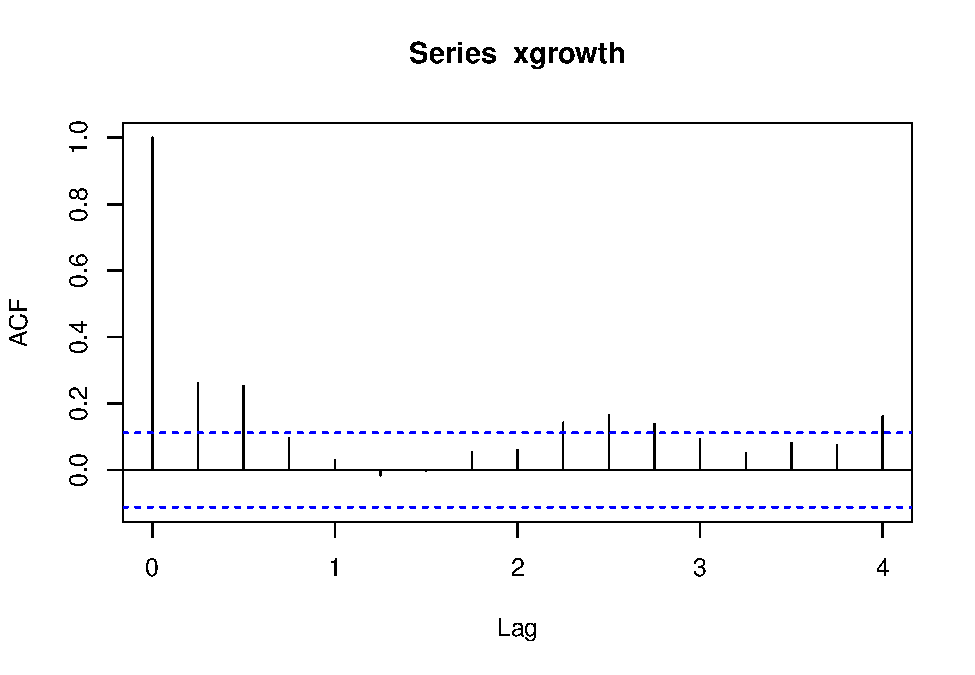
\includegraphics{_main_files/figure-latex/unnamed-chunk-15-1.pdf}

\begin{Shaded}
\begin{Highlighting}[]
\DocumentationTok{\#\# partial autocorrelation function}
\FunctionTok{pacf}\NormalTok{(xgrowth, }\AttributeTok{lag.max =} \DecValTok{16}\NormalTok{)}
\end{Highlighting}
\end{Shaded}

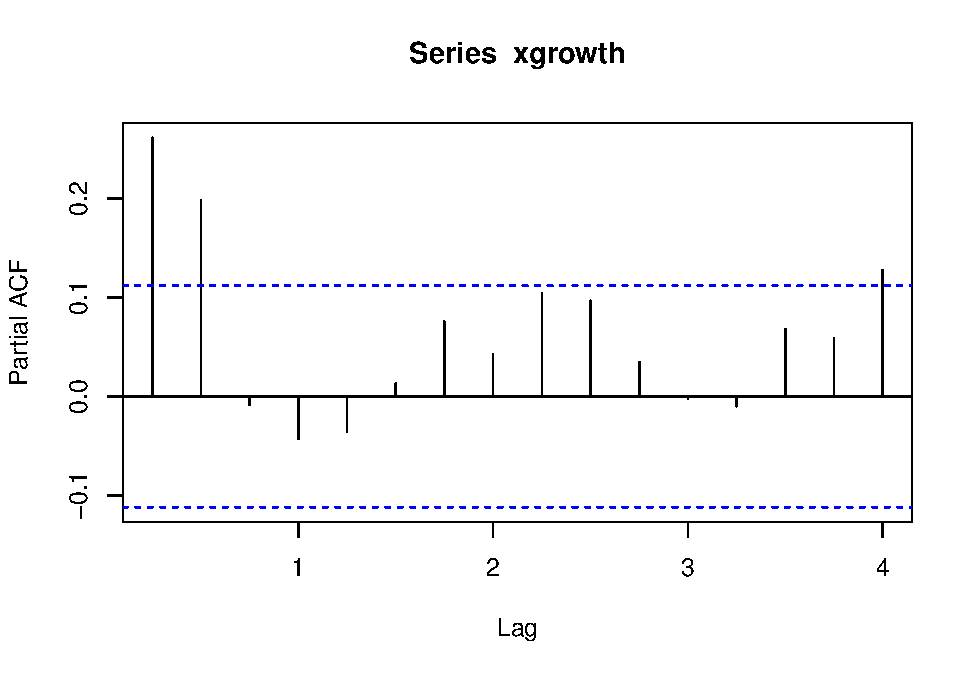
\includegraphics{_main_files/figure-latex/unnamed-chunk-16-1.pdf}

\hypertarget{hypothesis-testing}{%
\section{Hypothesis testing}\label{hypothesis-testing}}

In this section we use three testing procedures on the GDP growth data: the Augmented Dickey-Fuller test for stationarity, the Jarque-Bera test for normality and the t-test for the mean of a process.

\begin{Shaded}
\begin{Highlighting}[]
\DocumentationTok{\#\# Example 5: tests on GDP growth rates }
\FunctionTok{library}\NormalTok{(tseries)}

\DocumentationTok{\#\# stationarity: augmented Dickey{-}Fuller}
\FunctionTok{adf.test}\NormalTok{(x)}
\end{Highlighting}
\end{Shaded}

\begin{verbatim}
## 
##  Augmented Dickey-Fuller Test
## 
## data:  x
## Dickey-Fuller = 2.4611, Lag order = 6, p-value = 0.99
## alternative hypothesis: stationary
\end{verbatim}

\begin{Shaded}
\begin{Highlighting}[]
\FunctionTok{adf.test}\NormalTok{(xgrowth)}
\end{Highlighting}
\end{Shaded}

\begin{verbatim}
## 
##  Augmented Dickey-Fuller Test
## 
## data:  xgrowth
## Dickey-Fuller = -5.9064, Lag order = 6, p-value = 0.01
## alternative hypothesis: stationary
\end{verbatim}

\begin{Shaded}
\begin{Highlighting}[]
\DocumentationTok{\#\# normality: Jarque{-}Bera}
\FunctionTok{jarque.bera.test}\NormalTok{(xgrowth)}
\end{Highlighting}
\end{Shaded}

\begin{verbatim}
## 
##  Jarque Bera Test
## 
## data:  xgrowth
## X-squared = 2902.3, df = 2, p-value < 2.2e-16
\end{verbatim}

\begin{Shaded}
\begin{Highlighting}[]
\DocumentationTok{\#\# mean zero: t{-}test}
\NormalTok{sigmaLR }\OtherTok{\textless{}{-}} \FunctionTok{sum}\NormalTok{(}\FunctionTok{sapply}\NormalTok{(}\SpecialCharTok{{-}}\DecValTok{100}\SpecialCharTok{:}\DecValTok{100}\NormalTok{, gamma, }\AttributeTok{x =}\NormalTok{ xgrowth))}
\NormalTok{t\_stat  }\OtherTok{\textless{}{-}} \FunctionTok{mean}\NormalTok{(xgrowth)}\SpecialCharTok{/}\NormalTok{(}\FunctionTok{sqrt}\NormalTok{(sigmaLR}\SpecialCharTok{/}\NormalTok{t\_max))}
\NormalTok{p\_value }\OtherTok{\textless{}{-}}\NormalTok{ (}\DecValTok{1}\SpecialCharTok{{-}}\FunctionTok{pnorm}\NormalTok{(}\FunctionTok{abs}\NormalTok{(t\_stat)))}\SpecialCharTok{*}\DecValTok{2}
\CommentTok{\# plot(density(rnorm(1e6)), xlim = c({-}8, 8))}
\CommentTok{\# abline(v = t\_stat, col = "tomato", lwd = 2)}

\CommentTok{\# compare with unadjusted variance}
\CommentTok{\# t.test(xgrowth, mu = 0)}
\CommentTok{\# mean(xgrowth)/(sqrt((t\_max/(t\_max{-}1))*var(xgrowth)/t\_max)) \# for compatibility with t{-}test()}
\NormalTok{t\_stat\_unadjasted }\OtherTok{\textless{}{-}} \FunctionTok{mean}\NormalTok{(xgrowth)}\SpecialCharTok{/}\NormalTok{(}\FunctionTok{sqrt}\NormalTok{(}\FunctionTok{var}\NormalTok{(xgrowth)}\SpecialCharTok{/}\NormalTok{t\_max))}
\NormalTok{p\_value\_unadjasted }\OtherTok{\textless{}{-}}\NormalTok{ (}\DecValTok{1}\SpecialCharTok{{-}}\FunctionTok{pnorm}\NormalTok{(}\FunctionTok{abs}\NormalTok{(t\_stat\_unadjasted)))}\SpecialCharTok{*}\DecValTok{2}

\FunctionTok{rbind}\NormalTok{(}\AttributeTok{p\_value\_unadjasted =}\NormalTok{ p\_value\_unadjasted,}
      \AttributeTok{p\_value =}\NormalTok{ p\_value)}
\end{Highlighting}
\end{Shaded}

\begin{verbatim}
##                            [,1]
## p_value_unadjasted 0.000000e+00
## p_value            4.884981e-15
\end{verbatim}

\begin{Shaded}
\begin{Highlighting}[]
\CommentTok{\# We can study when does the adjustment really matters }
\CommentTok{\# using the results of the previous Monte Carlo simulation}

\DocumentationTok{\#\# Get variance and long{-}run variance}
\NormalTok{sigma }\OtherTok{\textless{}{-}} \FunctionTok{apply}\NormalTok{(x\_list, }\DecValTok{2}\NormalTok{, }\ControlFlowTok{function}\NormalTok{(x) }\FunctionTok{sqrt}\NormalTok{(}\FunctionTok{gamma}\NormalTok{(x, }\AttributeTok{k =} \DecValTok{0}\NormalTok{)}\SpecialCharTok{/}\FunctionTok{length}\NormalTok{(x)))}
\NormalTok{sigmaLR }\OtherTok{\textless{}{-}} \FunctionTok{apply}\NormalTok{(x\_list, }\DecValTok{2}\NormalTok{, }\ControlFlowTok{function}\NormalTok{(x) }\FunctionTok{sqrt}\NormalTok{(}\FunctionTok{sum}\NormalTok{(}\FunctionTok{sapply}\NormalTok{(}\SpecialCharTok{{-}}\DecValTok{3}\SpecialCharTok{:}\DecValTok{3}\NormalTok{, gamma, }\AttributeTok{x =}\NormalTok{ x))}\SpecialCharTok{/}\FunctionTok{length}\NormalTok{(x)))}

\DocumentationTok{\#\# Get adjusted and unadjusted t{-}statistics}
\NormalTok{t\_stat\_unadjasted }\OtherTok{\textless{}{-}}\NormalTok{ x\_means}\SpecialCharTok{/}\NormalTok{sigma}
\NormalTok{t\_stat }\OtherTok{\textless{}{-}}\NormalTok{ x\_means}\SpecialCharTok{/}\NormalTok{sigmaLR}

\DocumentationTok{\#\# Compute percentage of type{-}1 errors in the simulation}
\NormalTok{type1error }\OtherTok{\textless{}{-}} \FunctionTok{mean}\NormalTok{(}\FunctionTok{abs}\NormalTok{(t\_stat) }\SpecialCharTok{\textgreater{}} \FunctionTok{qnorm}\NormalTok{(}\FloatTok{0.975}\NormalTok{))}
\NormalTok{type1error\_unadjusted }\OtherTok{\textless{}{-}} \FunctionTok{mean}\NormalTok{(}\FunctionTok{abs}\NormalTok{(t\_stat\_unadjasted) }\SpecialCharTok{\textgreater{}} \FunctionTok{qnorm}\NormalTok{(}\FloatTok{0.975}\NormalTok{))}

\FunctionTok{rbind}\NormalTok{(}
  \AttributeTok{type1error =}\NormalTok{ type1error,}
  \AttributeTok{type1error\_unadjusted =}\NormalTok{ type1error\_unadjusted}
\NormalTok{)}
\end{Highlighting}
\end{Shaded}

\begin{verbatim}
##                         [,1]
## type1error            0.0569
## type1error_unadjusted 0.1716
\end{verbatim}

\begin{Shaded}
\begin{Highlighting}[]
\DocumentationTok{\#\# plot distributions of adjusted and unadjusted t{-}statistics}
\FunctionTok{hist}\NormalTok{(t\_stat\_unadjasted, }\AttributeTok{breaks =} \DecValTok{100}\NormalTok{, }\AttributeTok{freq =} \ConstantTok{FALSE}\NormalTok{, }\AttributeTok{col =} \StringTok{"tomato"}\NormalTok{, }
     \AttributeTok{ylim =} \FunctionTok{c}\NormalTok{(}\DecValTok{0}\NormalTok{, }\FloatTok{0.45}\NormalTok{), }\AttributeTok{xlim =} \FunctionTok{c}\NormalTok{(}\SpecialCharTok{{-}}\DecValTok{5}\NormalTok{, }\DecValTok{6}\NormalTok{), }\AttributeTok{xlab =} \StringTok{"t{-}stat"}\NormalTok{, }
     \AttributeTok{main =} \StringTok{"Distribution of the t{-}statistic in Monte Carlo simulation"}\NormalTok{)}
\FunctionTok{hist}\NormalTok{(t\_stat, }\AttributeTok{breaks =} \DecValTok{100}\NormalTok{, }\AttributeTok{freq =} \ConstantTok{FALSE}\NormalTok{, }\AttributeTok{add =} \ConstantTok{TRUE}\NormalTok{, }\AttributeTok{col =} \StringTok{"lightgreen"}\NormalTok{)}
\FunctionTok{lines}\NormalTok{(}\FunctionTok{density}\NormalTok{(}\FunctionTok{rnorm}\NormalTok{(}\FloatTok{1e6}\NormalTok{, }\AttributeTok{mean =} \DecValTok{0}\NormalTok{, }\AttributeTok{sd =} \DecValTok{1}\NormalTok{)), }\AttributeTok{lwd =} \DecValTok{4}\NormalTok{, }\AttributeTok{col =} \StringTok{"black"}\NormalTok{)}
\FunctionTok{legend}\NormalTok{(}\StringTok{"topright"}\NormalTok{, }\FunctionTok{c}\NormalTok{(}\StringTok{"Unadjusted"}\NormalTok{, }\StringTok{"Adjusted"}\NormalTok{), }\AttributeTok{col=}\FunctionTok{c}\NormalTok{(}\StringTok{"tomato"}\NormalTok{, }\StringTok{"lightgreen"}\NormalTok{), }\AttributeTok{lwd=}\DecValTok{6}\NormalTok{)}
\FunctionTok{abline}\NormalTok{(}\AttributeTok{v =} \FunctionTok{qnorm}\NormalTok{(}\FunctionTok{c}\NormalTok{(}\FloatTok{0.025}\NormalTok{, }\FloatTok{0.975}\NormalTok{)), }\AttributeTok{lty =} \DecValTok{2}\NormalTok{, }\AttributeTok{lwd =} \DecValTok{2}\NormalTok{)}
\FunctionTok{text}\NormalTok{(}\AttributeTok{x=}\FunctionTok{c}\NormalTok{(}\FloatTok{6.5}\NormalTok{, }\FloatTok{6.5}\NormalTok{), }\AttributeTok{y=}\FunctionTok{c}\NormalTok{(}\FloatTok{0.3}\NormalTok{, }\FloatTok{0.25}\NormalTok{), }
     \AttributeTok{labels=}\FunctionTok{c}\NormalTok{(}\FunctionTok{paste0}\NormalTok{(}\StringTok{"Type 1 error: "}\NormalTok{, }\FunctionTok{round}\NormalTok{(type1error\_unadjusted}\SpecialCharTok{*}\DecValTok{100}\NormalTok{, }\DecValTok{1}\NormalTok{), }\StringTok{"\%"}\NormalTok{),}
              \FunctionTok{paste0}\NormalTok{(}\StringTok{"Type 1 error adjusted: "}\NormalTok{, }\FunctionTok{round}\NormalTok{(type1error}\SpecialCharTok{*}\DecValTok{100}\NormalTok{, }\DecValTok{1}\NormalTok{), }\StringTok{"\%"}\NormalTok{)), }
     \AttributeTok{col=}\FunctionTok{c}\NormalTok{(}\StringTok{"tomato"}\NormalTok{, }\StringTok{"lightgreen"}\NormalTok{), }\AttributeTok{pos =} \DecValTok{2}\NormalTok{)}
\end{Highlighting}
\end{Shaded}

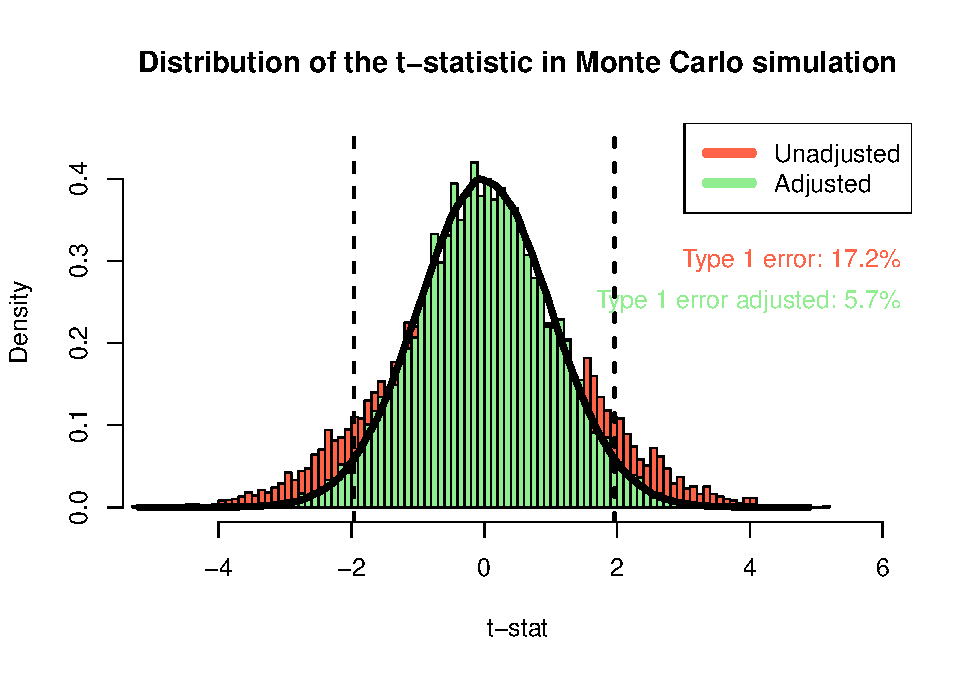
\includegraphics{_main_files/figure-latex/unnamed-chunk-19-1.pdf}

  \bibliography{book.bib,packages.bib}

\end{document}
